\begin{center}
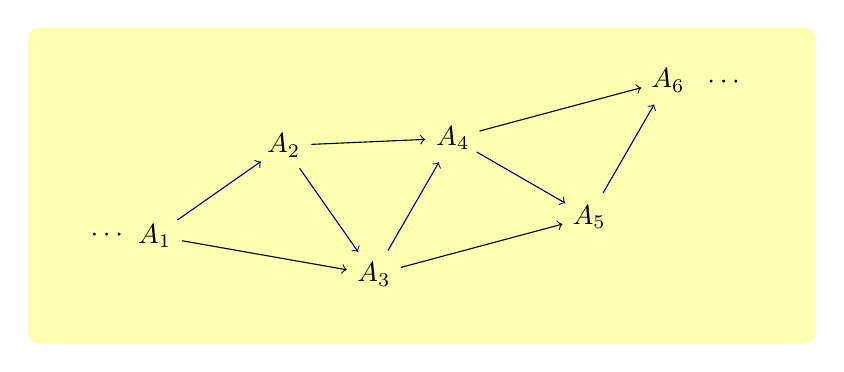
\begin{tikzpicture}
\fill[draw, Yellow!30, rounded corners]
(-5, -2) rectangle (5, 2);
\node at (-4.3,1.5) {$\cc$};
\pgfmathsetmacro{\r}{2}

\begin{scope}[xshift = -1.25cm, rotate = -10]
\coordinate (A1) at (-2,-1);
\pgfmathsetmacro{\x}{-2 + \r*cos(45 )};
\pgfmathsetmacro{\y}{-1 + \r*sin(45 )};
\coordinate (A2) at (\x,\y);
\pgfmathsetmacro{\x}{\x + \r*cos(-45 )};
\pgfmathsetmacro{\y}{\y + \r*sin(-45 )};
\coordinate (A3) at (\x,\y);
\pgfmathsetmacro{\x}{\x + \r*cos(70 )};
\pgfmathsetmacro{\y}{\y + \r*sin(70 )};
\coordinate (A4) at (\x,\y);
\pgfmathsetmacro{\x}{\x + \r*cos(-20 )};
\pgfmathsetmacro{\y}{\y + \r*sin(-20 )};
\coordinate (A5) at (\x,\y);
\pgfmathsetmacro{\x}{\x + \r*cos(70 )};
\pgfmathsetmacro{\y}{\y + \r*sin(70 )};
\coordinate (A6) at (\x,\y);

\foreach \n in {1,2,3,4,5,6}{
\node at (A\n) {$A_{\n}$};
}
\node at ([xshift = -0.6cm, yshift= -0.1cm]A1) {$\cdots$};
\node at ([xshift = 0.7cm, yshift =0.1cm]A6) {$\cdots$};

\draw[->, shorten >= 10pt, shorten <=10pt, NavyBlue] (A1)--(A2);
\draw[->, shorten >= 10pt, shorten <=10pt,  NavyBlue] (A2)--(A3);
\draw[->, shorten >= 10pt, shorten <=10pt,  NavyBlue] (A3)--(A4);
\draw[->, shorten >= 10pt, shorten <=10pt,  NavyBlue] (A4)--(A5);
\draw[->, shorten >= 10pt, shorten <=10pt,  NavyBlue] (A5)--(A6);

\draw[->, shorten >= 10pt, shorten <=10pt] (A1)--(A3);
\draw[->, shorten >= 10pt, shorten <=10pt] (A2)--(A4);
\draw[->, shorten >= 10pt, shorten <=10pt] (A3)--(A5);
\draw[->, shorten >= 10pt, shorten <=10pt] (A4)--(A6);

\end{scope}
\end{tikzpicture}
\end{center}